\documentclass{article}
\usepackage[utf8]{inputenc}
\usepackage{geometry}
\usepackage{graphicx}
\usepackage{amsmath}
\usepackage{amsfonts}
\usepackage{amsthm}
\usepackage{amssymb}
\usepackage[most]{tcolorbox}
\usepackage{array}
\usepackage{latexsym}
\usepackage{alltt}
\usepackage{hyperref}
\usepackage{color}
\usepackage{float}
\usepackage{pdfpages}
\usepackage{algpseudocode}
\usepackage{multicol}
\usepackage{multirow}
\usepackage{caption}
\usepackage{xparse}
\usepackage{setspace}
\usepackage{enumitem}
\usepackage{pdflscape}
% \usepackage{parskip} % No indent for each paragraph if it is not commented
\usepackage{blindtext}
\usepackage{forest}
\usepackage[newfloat]{minted}


\geometry
{
  a4paper,
  left=12mm,
  right=12mm,
  top=12mm,
  bottom=15mm,
}

% mybox
\newtcolorbox{mybox}[3][]
{
  colframe = #2!25,
  colback  = #2!10,
  coltitle = #2!20!black,  
  title    = {#3},
  #1,
}

\definecolor{bg}{rgb}{0.95,0.95,0.95}
\setminted
{
  mathescape=true,
  xleftmargin=\parindent,
  bgcolor=bg
}

% \newenvironment{code}{\captionsetup{type=listing}}{}
\SetupFloatingEnvironment{listing}{name=Code}

\usetikzlibrary{patterns,positioning,fit,arrows,matrix,calc,shapes.geometric,shapes.multipart,decorations.pathreplacing}

% New environments that use mybox
\newcounter{example}[section]
\newenvironment{example}[1]{\begin{mybox}[breakable]{green}{\refstepcounter{example}\textbf{Example \thesection.\theexample #1}}}{\end{mybox}}

\newcounter{definition}[section]
\newenvironment{definition}[1]{\refstepcounter{definition}\begin{mybox}[breakable]{blue}{\textbf{Definition \thesection.\thedefinition #1}}}{\end{mybox}}

\newcounter{theorem}[section]
\newenvironment{theorem}[1]{\begin{mybox}{red}{\refstepcounter{theorem}\textbf{Theorem \thesection.\thetheorem #1}}}{\end{mybox}}

\newenvironment{formula}[1]{\begin{mybox}{cyan}{\textbf{#1}}}{\end{mybox}}

% Changing maketitle
\makeatletter         
\renewcommand\maketitle{
{\raggedright % Note the extra {
\begin{center}
{\Large \bfseries \@title}\\[2ex] 
{\large \@author \ - \@date}\\[2ex]
\end{center}}} % Note the extra }
\makeatother

% \onehalfspacing % adjust spacing
\setlength{\parskip}{0.5\baselineskip}

% macros
\newcommand{\prob}[1]{\textbf{\textit{P}}\left\{#1\right\}}
\newcommand{\expc}[1]{\mathbf{E}\left(#1\right)}
\newcommand{\expcs}[1]{\mathbf{E}^2\left(#1\right)}
\newcommand{\var}[1]{\text{Var}\left( #1 \right)}
\newcommand{\ra}{\rightarrow}
\newcommand{\Ra}{\Rightarrow}

\NewDocumentCommand{\dsum}{%
    e{^_}
}{%
  {% 
    \displaystyle\sum
    \IfValueT{#1}{^{#1}}
    \IfValueT{#2}{_{#2}}
  }
}%

% maketitle variables
\title{CENG 242 - Chapter 3: Variables and Storage}
\author{Burak Metehan Tunçel}
\date{May 2022}

\begin{document}

\maketitle

\begin{multicols*}{2}
\setlength{\columnsep}{1.5cm}
\setlength{\columnseprule}{0.2pt}

\section{Variables and Storage}

The variables of imperative programs \textit{do not} behave like mathematical variables. (A mathematical variable stands for a fixed but unknown value; there is no implication of change over time.) The variables of functional and logic programs \textit{do} behave like mathematical variables.

In imperative (and object-oriented and concurrent) programming languages, a \textit{\textbf{variable}} is a container for a value, and may be \textit{inspected} and \textit{updated} as often as desired.

To understand how the variables of imperative programs really do behave, we need some notion of \textit{\textbf{storage}}. We use an abstract model of storage that is simple but adequate:
\begin{itemize}
  \item A store is a collection of \textit{\textbf{storage cells}}, each of which has a unique address.
  \item Each storage cell has a current \textit{status}, which is either \textit{allocated} or \textit{unallocated}. Each allocated storage cell has a current \textit{content}, which is either a \textit{storable value} or \textit{undefined}.
\end{itemize}

\begin{figure}[H]
  \centering
  \includegraphics[width=.8\linewidth]{img/fig-3.1.png}
  \caption{An abstract storage model.}
\end{figure}

In terms of this storage model, we can view a variable as a container consisting of one or more storage cells. More precisely:
\begin{itemize}
  \item A \textit{\textbf{simple variable}} occupies a single allocated storage cell.
  \item A \textit{\textbf{composite variable}} occupies a group of contiguous allocated storage cells.
\end{itemize}

A \textit{\textbf{storable}} value is one that can be stored in a single storage cell. Each programming language counts certain types of values as storable:
\begin{itemize}
  \item \texttt{C++}'s storable values are primitive values and pointers. (Structures, arrays, unions, and objects are not storable, since none of these can be stored in a single storage cell. Functions also are not storable, since they cannot be stored at all. However, pointers to all of these things are storable.)
  \item \texttt{JAVA}'s storable values are primitive values and pointers to objects. (Objects themselves are not storable, but every object is implicitly accessed through a pointer.)
\end{itemize}

As a rule of thumb, most programming languages count \textit{primitive values and pointers as storable, but not composite values.}

As an example, in the \hyperref[code:code-1]{code 1}:
\begin{itemize}
  \item When function is called, cells are initially unallocated.
  \item In line 2, cell is allocated/undefined. It is ready to use but value is unknown.
  \item In line 4, it is storable.
  \item In line 6, After the including block terminates, the cell is again unallocated.
\end{itemize}

\begin{listing}[H]
\begin{minted}[linenos, xleftmargin=20pt]{cpp}
void f() {
  int x;
  ...
  x=5;
  ...
  return;
}

f();
\end{minted}
\caption{}
\label{code:code-1}
\end{listing}


\section{Simple and Composite Variables}

\subsection{Simple Variables}

A \textit{\textbf{simple variable}} is a variable that may contain a storable value. \textit{Each simple variable occupies a single storage cell}.

\subsection{Composite Variables}

A \textit{\textbf{composite variable}} is a variable of a composite type. \textit{Each composite variable occupies a group of contiguous storage cells}.

\subsubsection{Total vs Selective Update}

A composite variable may be updated either \textit{in a single step} or \textit{in several steps}, one component at a time. \textit{\textbf{Total update}} of a composite variable means updating it with a new (composite) value in a single step. \textit{\textbf{Selective update}} of a composite variable means updating a single component.

\begin{listing}[H]
\begin{minted}[]{c}
struct Complex { double x, y; } a, b;
...
a = b; // Total update
a.x = b.y * a.x; // Selective update
\end{minted}
\caption{}
\label{code:code-2}
\end{listing}

\subsubsection{Static vs Dynamic vs Flexible Arrays}

We can view an array variable as a mapping from an index range to a group of component variables. How and when a given array variable's index range is determined can be changed. There are several possibilities:
\begin{itemize}
  \item the index range might be fixed at compile-time
  \item the index range might be fixed at run-time when the array variable is created
  \item the index range might not be fixed at all
\end{itemize}

A \textit{\textbf{static array}} is an array variable whose index range is fixed at compile-time. In other words, the program code determines the index range.

A \textit{\textbf{dynamic array}} is an array variable whose index range is fixed at the time when the array variable is created.

A \textit{\textbf{flexible array}} is an array variable whose index range is not fixed at all. A flexible array's index range may be changed when a new array value is assigned to it.


\section{Copy Semantics vs Reference Semantics}

When a program assigns a composite value to a variable of the same type, what happens depends on the language. There are in fact two distinct possibilities:
\begin{itemize}
  \item \textit{\textbf{Copy semantics}}. The assignment copies all components of the composite value into the corresponding components of the composite variable.
  \item \textit{\textbf{Reference semantics}}. The assignment makes the composite variable contain a pointer (or reference) to the composite value.
\end{itemize}

Copy semantics is adopted by \texttt{C} and \texttt{C++}. However, programmers can also achieve the effect of reference semantics by using explicit pointers.

\texttt{JAVA} adopts copy semantics for primitive values, and reference semantics for objects. However, programmers can achieve the effect of copy semantics even for objects by using the clone method.

The semantics of the \textit{equality test} operation in any programming language should be consistent with the semantics of assignment. This enables the programmer to assume that, immediately after an assignment of  $V_1$ to $V_2$, $V_1$ is equal to $V_2$, regardless of whether copy or reference semantics is used. It follows that the equality test operation should behave as follows:
\begin{itemize}
  \item \textit{Copy semantics}. The equality test operation should test whether corresponding components of the two composite values are equal.
  \item \textit{Reference semantics}. The equality test operation should test whether the pointers to the two composite values are equal (i.e., whether they point to the same variable)
\end{itemize}

\textit{Copy semantics is slower than reference semantics. Reference semantics cause problems from storage sharing (all operations effect both variables), deallocation of one makes the other invalid.}


\section{Lifetime}

Every variable is \textit{\textbf{created}} (or \textit{allocated}) at some definite time, and \textit{\textbf{destroyed}} (or \textit{deallocated}) at some later time when it is no longer needed. \textit{The interval between creation and destruction} of a variable is called its \textit{\textbf{lifetime}}.

The concept of lifetime is pragmatically important. A variable needs to occupy storage cells only during its lifetime. We can classify variables according to their lifetimes:
\begin{itemize}
  \item A \textit{\textbf{global variable}}'s lifetime is \textit{the program's run-time}.
  \item A \textit{\textbf{local variable}}'s lifetime is \textit{an activation of a block}.
  \item A \textit{\textbf{heap variable}}'s lifetime is \textit{arbitrary, but is bounded by the program's run-time.}
  \item A \textit{\textbf{persistent variable}}'s lifetime is \textit{arbitrary, and may transcend the run-time of any particular program}.
\end{itemize}

\subsection{Global and Local Variables}

A \textit{\textbf{global variable}} is one that is declared for use throughout the program. A global variable's lifetime is the program's entire run-time: \textit{the variable is created when the program starts, and is destroyed when the program stops}.

A \textit{\textbf{local variable}} is one that is declared within a block, for use only within that block. A lifetime of a local variable is an activation of the block containing that variable's declaration: \textit{the variable is created on entry to the block, and is destroyed on exit from the block.}

A \textit{\textbf{block}} is a program construct that includes local declarations. In all programming languages, the body of a procedure is a block. An \textit{\textbf{activation}} of a block is the time interval during which that block is being executed. In particular, \textit{an activation of a procedure is the time interval between call and return}. During a single run of the program \textit{a block may be activated several times, and so a local variable may have several lifetimes}.

A local variable \textit{cannot retain its content over successive activations of the block} in which it is declared. In some programming languages, a variable may be initialized as part of its declaration. But if a variable is not initialized, its content is \textit{undefined}, \textit{not} the value it might have contained in a previous activation of the block.

Some programming languages (such as \texttt{C}) allow a variable to be declared as a \textit{\textbf{static variable}}, which defines its lifetime to be the program's entire run-time (even if the variable is declared inside a block). Thus static variables have the same lifetime as global variables. Although this feature addresses a genuine need, there are better ways to achieve the same effect, such as class variables in object-oriented languages.

\end{multicols*}

\begin{multicols}{2}
\setlength{\columnsep}{1.5cm}
\setlength{\columnseprule}{0.2pt}

\subsection{Heap Variables}

A \textit{\textbf{heap variable}} is one that can be created, and destroyed, at any time during the program's run-time. A heap variable is created by an expression or command. \textit{It is anonymous, and is accessed through a pointer. (By contrast, a global or local variable is created by a declaration, and has an identifier.)} The lifetimes of heap variables follow no particular pattern. 

Pointers are first-class values, and thus may be stored, used as components of composite values, and so on. 

An \textit{\textbf{allocator}} is an operation that creates a heap variable, yielding a pointer to that heap variable. In \texttt{C++} and \texttt{JAVA}, an expression of the form ``\texttt{\textbf{new}} ...'' is an allocator. (In \texttt{C}, \texttt{malloc()}.)

A \textit{\textbf{deallocator}} is an operation that destroys a given heap variable. \texttt{C++}'s deallocator is a command of the form ``\texttt{\textbf{delete}} ...''. \texttt{JAVA} has no deallocator at all. (In \texttt{C}, \texttt{free()}.) Deallocators are unsafe, since any remaining pointers to a destroyed heap variable become \hyperref[sec:dangling-pointers]{\textit{dangling pointers}}.

A heap variable remains \textit{\textbf{reachable}} as long as it can be accessed by following pointers from a global or local variable. A heap variable's lifetime extends from its creation until it is destroyed or it becomes unreachable.

Sometimes, operating system tolerates dangling references. However, sometimes, it generates run-time erros like ``protection fault'' or ``segmentation fault'' are generated.

\subsubsection{Garbage Variables}

\textit{\textbf{Garbage variables}} are the variables with lifetime still continue but there is no way to access.

\begin{minted}{c}
...
char *p, *q;
p = malloc(10);
p = q;
...
void f() {
  char *p;
  p= malloc(10); ...
  return;
}

f ();
\end{minted}

When the pointer value is lost or lifetime of the pointer is
over, heap variable is unaccessible. (\texttt{*p} in examples)

\subsubsection{Garbage Collection}

A solution to dangling reference and garbage problem is garbage collection. Garbage collection (GC) is a form of automatic memory management. The garbage collector attempts to reclaim memory which was allocated by the program, but is no longer referenced-also called garbage. In other words, PL does management of heap variable deallocation
automatically. \texttt{Java, Lisp, ML, Haskell} and most functional languages provide garbage collection.

Also, Calls like free() or delete does not exist. Language runtime needs to:
\begin{itemize}
  \item Keep a reference counter on each reference, initially 1
  \item Increment counter on each new assignment
  \item Decrement counter at the end of the reference lifetime
  \item Decrement counter at the overwritten/lost references
  \item Do all these operations recursively on composite values.
  \item When reference count gets 0, deallocate the heap variable
\end{itemize}

Garbage collector deallocates heap variables having a reference count 0. Since it may delay execution of tasks, GC is not immediately done. GC usually works in a separate thread, in low priority, works when CPU is idle.

Another but too restrictive solution to garbage is that \textit{reference cannot be assigned to a longer lifetime variable}. Local variable references cannot be assigned to global reference/pointer.

\subsection{Persistent Variables}

\textit{\textbf{Files}} may be seen as composite variables. In particular, a \textit{\textbf{sequential file}} is a sequence of components, and a direct file is (in effect) an array of components.

Usually files contain large bodies of long-lived data: they are \textit{persistent}. A \textit{\textbf{persistent variable}} is one whose lifetime transcends an activation of any particular program. By contrast, a \textit{\textbf{transient variable}} is one whose lifetime is bounded by the activation of the program that created it. \textit{Global, local, and heap variables are transient.}

There are certain analogies between persistent variables and transient variables. Persistent variables usually have arbitrary lifetimes, like heap variables; but some systems also allow persistent variables to have nested lifetimes, like local variables. Just as transient variables occupy primary storage, persistent variables occupy secondary storage.

\subsubsection{Type Completeness Principle}

The \textit{\textbf{Type Completeness Principle}} suggests that all the types of the programming language should be available for both transient and persistent variables. A language applying this principle would be simplified by having no special file types, and no special commands or procedures for reading/writing data from/to files. The programmer would be spared the unprofitable effort of converting data from a persistent data type to a transient data type on input, and vice versa on output.

\end{multicols}

\newpage

\subsection{Examples}

%%%%%%%%%%%%%%% Example of Global and Local Variables %%%%%%%%%%%%%%%
%% Taken from the slides of Onur Tolga Şehitoğlu %%

\begin{multicols}{2}

%% Column 1 %%
\begin{listing}[H]

\begin{minted}{cpp}
double x;

int h( int n) {
  int a;
  if (n <1) return 1;
  else return h(n -1);
}

void g() {
  int x;
  int b;
  ...
}

int f () {
  double z ;
  ...
  g ();
  ...
}

int main () {
  double k;
  f ();
  ...
  h(1);
  ...;
  return 0;
}
\end{minted}

\caption{Example of Global and Local Variables.}
\label{code:code-3}
  
\end{listing}

%%%%%%%%%%%%%%%%%%%%%%%%%%
\columnbreak
%%%%%%%%%%%%%%%%%%%%%%%%%%

%% Column 2 %%
%% Taken from the slides of Onur Tolga Şehitoğlu %%

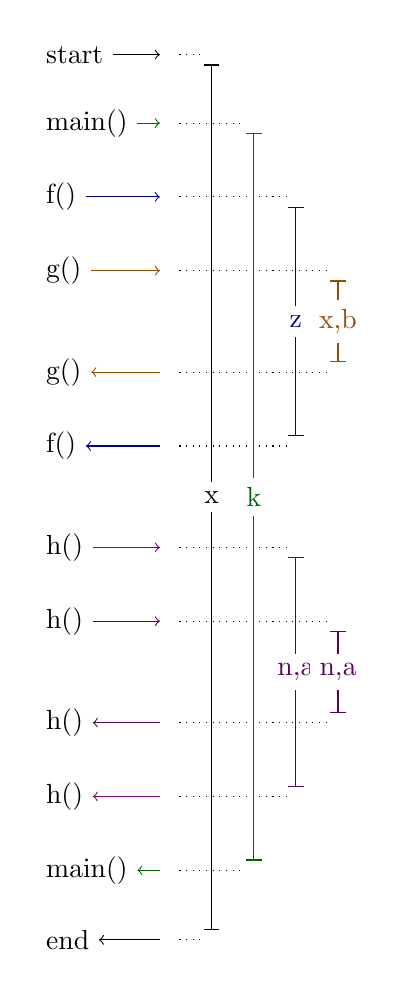
\begin{tikzpicture} 
\matrix [column sep=3mm,ampersand replacement=\&] {
\node [right](bb) {start}; \& \node (dbb) {}; \& \node (kb) {};  \\[1em]
\node [right](bm) {main()}; \& \node (dbm) {}; \&  \& \node (mb) {}; \\[1em]
\node [right](bf) {f()}; \& \node (dbf) {}; \&  \&  \& \node (fb) {}; \\[1em]
\node [right](bg) {g()}; \& \node (dbg) {}; \&  \&  \& \& \node (gb) {}; \\[2em]
\node [right](cg) {g()}; \& \node (dcg) {}; \&  \&  \& \& \node (gc) {}; \\[1em]
\node [right](cf) {f()}; \& \node (dcf) {}; \&  \&  \& \node (fc) {}; \\[2em]
\node [right](bh1) {h()}; \& \node (dbh1) {}; \&  \&  \& \node (h1b) {}; \\[1em]
\node [right](bh2) {h()}; \& \node (dbh2) {}; \&  \&  \& \& \node (h2b) {}; \\[2em]
\node [right](ch2) {h()}; \& \node (dch2) {}; \&  \&  \& \& \node (h2c) {}; \\[1em]
\node [right](ch1) {h()}; \& \node (dch1) {}; \&  \&  \& \node (h1c) {}; \\[1em]
\node [right](cm) {main()}; \& \node (dcm) {}; \&  \& \node (mc) {}; \\[1em]
\node [right](cb) {end}; \& \node (dcb) {}; \& \node (kc) {};  \\[1em]
};
\draw [->] (bb) -- (dbb);	\draw [dotted] (dbb) -- (kb);
\draw [green!40!black,->] (bm) -- (dbm);  		\draw [dotted] (dbm) -- (mb);
\draw [blue!60!black,->] (bf) -- (dbf);   		\draw [dotted] (dbf) -- (fb);
\draw [orange!60!black,->] (bg) -- (dbg);    		\draw [dotted] (dbg) -- (gb);
\draw [orange!60!black,<-] (cg) -- (dcg);  		\draw [dotted] (dcg) -- (gc);
\draw [blue!60!black,<-] (cf) -- (dcf);   		\draw [dotted] (dcf) -- (fc);
\draw [green!40!black,<-] (cm) -- (dcm);  		\draw [dotted] (dcm) -- (mc);
\draw [violet,->] (bh1) -- (dbh1);   		\draw [dotted] (dbh1) -- (h1b);
\draw [violet!70!black,->] (bh2) -- (dbh2);  		\draw [dotted] (dbh2) -- (h2b);
\draw [violet!70!black,<-] (ch2) -- (dch2);  		\draw [dotted] (dch2) -- (h2c);
\draw [violet,<-] (ch1) -- (dch1);   		\draw [dotted] (dch1) -- (h1c);
\draw [<-] (cb) -- (dcb);	\draw [dotted] (dcb) -- (kc);
\draw [|-|] (kb) -- node [fill=white] {x} (kc);
\draw [|-|,green!40!black] (mb) -- node [fill=white] {k} (mc);
\draw [|-|,blue!60!black] (fb) -- node [fill=white] {z} (fc);
\draw [|-|,orange!60!black] (gb) -- node [fill=white] {x,b} (gc);
\draw [|-|,violet!70!black] (h1b) -- node [fill=white] {n,a} (h1c);
\draw [|-|,violet!70!black] (h2b) -- node [fill=white] {n,a} (h2c);
\end{tikzpicture}

\end{multicols}
  
%%%%%%%%%%%%%%%%%%%%%%%%%%%%%%%%%%%%%%%%%%%%%%%%%%%%%%%%%%%%%%%%%%%%%

%%%%%%%%%%%%%%% Example of Heap Variables %%%%%%%%%%%%%%%

\begin{listing}[H]

\begin{minted}{c}
double *p;

int h() { ...
}

void g() { ...
  p = malloc(sizeof(double));
}

int f() { ...
  g(); ...
}

int main() { ...
  f();    ...
  h();    ...;
  free(p); ...
}
\end{minted}

\caption{Example of Heap Variables.}
\label{code:code-4}

\end{listing}

\begin{center}
  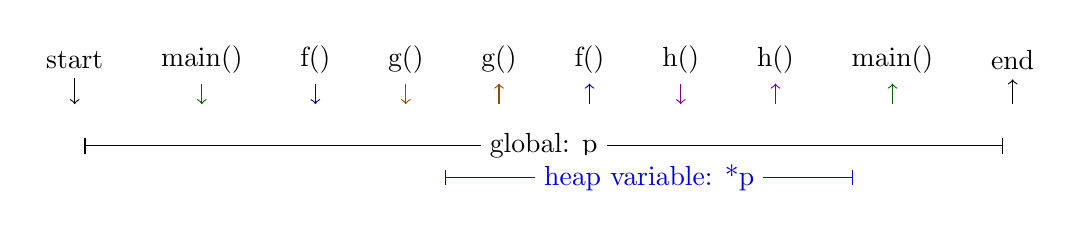
\begin{tikzpicture}
    \matrix [ampersand replacement=\&, column sep=5mm, row sep=1mm] {
    \node (bb) {start}; \& \node (bm) {main()}; \& \node (bf) {f()}; \& 
    \node (bg) {g()}; \& \node (cg) {g()}; \& \node (cf) {f()}; \& 
    \node (bh1) {h()}; \& 
    \node (ch1) {h()}; \& \node (cm) {main()}; \& \node (cb) {end}; \\[.5em]
    \node (dbb) {}; \& \node (dbm) {}; \& \node (dbf) {}; \& 
    \node (dbg) {}; \& \node (dcg) {}; \& \node (dcf) {}; \& 
    \node (dbh1) {}; \&
    \node (dch1) {}; \& \node (dcm) {}; \& \node (dcb) {}; \\[.2em]
    \node (kb) {} ;\& \& \& \& \& \& \& \& \& \node (kc) {}; \\[.2em] 
    \& \& \& \node (yb) {}; \& \& \& \&  \& \node (yc) {}; \& \\
    };
    \draw [->] (bb) -- (dbb);
    \draw [|-|] (kb) -- node [fill=white] {global: p} (kc);
    \draw [blue!90!black,|-|] (yb) +(5mm,0) -- node [fill=white] {heap variable: *p} ($(yc) - (5mm,0)$);
    \draw [green!40!black,->] (bm) -- (dbm); 
    \draw [blue!60!black,->] (bf) -- (dbf); 
    \draw [orange!60!black,->] (bg) -- (dbg);  
    \draw [orange!60!black,<-] (cg) -- (dcg);
    \draw [blue!60!black,<-] (cf) -- (dcf); 
    \draw [violet,->] (bh1) -- (dbh1); 
    \draw [violet,<-] (ch1) -- (dch1); 
    \draw [green!40!black,<-] (cm) -- (dcm);
    \draw [<-] (cb) -- (dcb);
  \end{tikzpicture}
\end{center}
  
%%%%%%%%%%%%%%%%%%%%%%%%%%%%%%%%%%%%%%%%%%%%%%%%%%%%%%%%%

\begin{multicols*}{2}
\setlength{\columnsep}{1.5cm}
\setlength{\columnseprule}{0.2pt}


\section{Memory Management}
\label{sec:memory-management}

Memory manamegement of variables involves architecture, operating system, language runtime and the compiler. A typical OS divides memory in sections (segments):
\begin{itemize}
  \item \textit{\textbf{Stack section:}} run time stack
  \item \textit{\textbf{Heap section:}} heap variables
  \item \textit{\textbf{Data section:}} global variables
  \item \textit{\textbf{Code section:}} executable instructions, read only.
\end{itemize}
\textit{Global variables} are fixed at compile time and they are put in data section. \textit{Heap variables} are stored in the dynamic data structures in heap section. \textit{Heap section grows and shrinks as new variables are allocated and deallocated}. Heap section is maintained by language runtime. For \texttt{C}, it is \texttt{libc}.

\subsection{Local Variables}

Local variables can have multiple instances alive in case of recursion. For recursive calls of a function, there should be multiple instances of a variable and compiled code should know where it is depending on the current call state. The solution is to use \textit{\textbf{run-time stack}}. Each function call will introduce an \textit{\textbf{activation record}} to store its local context. It is also called \textbf{stack frame}, \textbf{activation frame}.

In a typical architecture, \textit{\textbf{activation record}} contains:
\begin{itemize}
  \item \textit{\textbf{Return address}}. Address of the next instruction after the caller.
  \item \textit{\textbf{Parameter values}}.
  \item \textit{A reserved area for local variables}.
\end{itemize}

\subsection{Function Call}

When a function is called:
\begin{itemize}
  \item \textbf{Caller Side}:
    \begin{itemize}
      \item Push parameters
      \item Push return address and jump to function code start (usually a single CPU instruction like callq )
    \end{itemize}
  
    \item \textbf{Function entry}:
      \begin{itemize}
        \item Set base pointer to current stack pointer
        \item Advance stack pointer to size of local variables
      \end{itemize}
    
    \item Function body can access all local variables relative to base pointer
    
    \item \textbf{Function return}:
      \begin{itemize}
        \item Set stack pointer to base pointer
        \item Pop return address and jump to return address (single CPU instruction like retq)
      \end{itemize}
    
    \item \textbf{Caller side after return}:
      \begin{itemize}
        \item Recover stack pointer (remove parameters on stack)
        \item Get and use return value if exists (typically from a register)
      \end{itemize}
\end{itemize}

All locals and parameters have the same offset from base pointer. Recursive calls execute same instructions.

\begin{itemize}
  \item Order of values in the activation record may differ for different
  languages.
  \item Registers are used for passing primitive value parameters instead of stack.
  \item Garbage collecting languages keep references on stack with actual variables on heap.
  \item Languages returning nested functions as first order values require more complicated mechanisms.
\end{itemize}

% \end{multicols*}

% \subsection{Examples}

% %%%%%%%%%%%%%%%%%%%%%%%%%%%%%%%%%%%%%%%%%%%%%%%%%%%%%%%%%%%%%%%%%

% %%%% Example of Activation Record %%%%

% \begin{multicols}{2}

% %% Column 1 %%
% \begin{listing}[H]

% \begin{minted}{c}
% int f(short a, int b) {
%   char tmp[10];
%   ...
%   return a + b;
% }

% int g(int x) {
%   int tmp, p;
%   ...
%   tmp = f(x, x+1);
%   ...
%   return tmp + p;
% }

% int main() {
%   return g(4);
% }
% \end{minted}
  
% \caption{Example of Activation Record.}
% \label{code:code-5}
  
% \end{listing}

% %% Column 2 %%
% \begin{center}

% \begin{tikzpicture}
%       [stack/.style={rectangle split, rectangle split parts=#1,draw,
%       text width=10em}]
%   \node [stack=10, rectangle split part fill={white,blue!40!white,blue!40!white,blue!40!white,
%       green!40!white, green!40!white, green!40!white,
%       orange!40!white, orange!40!white, orange!40!white}] (stk) {
%   \nodepart{one} \rule{0pt}{3em}
%   \nodepart{two} locals to f():\\
%                   tmp,10 bytes
%   \nodepart{three} return adress:\\
%           end of line 9
%   \nodepart{four} parameters of f():\\
%           a=4, b=5 (6 bytes)
%   \nodepart{five} locals to g():\\
%           none
%   \nodepart{six} return adress:\\
%           end of line 14
%   \nodepart{seven} parameters of g():\\
%           x = 4
%   \nodepart{eight} locals to main():\\
%   \nodepart{nine} return adress:\\
%             program exit code
%   \nodepart{ten} parameters of main():\\
%   };
%   \draw [decorate,thick,decoration={brace,mirror,raise=5pt}] (stk.text split west) to (stk.four split west); 
%   \draw [decorate,thick,decoration={brace,mirror,raise=5pt}] (stk.four split west) to (stk.seven split west); 
%   \draw [decorate,thick,decoration={brace,mirror,raise=5pt}] (stk.seven split west) to (stk.south west); 
%   \node [left=of stk.three,rotate=90,anchor=center,yshift=-5mm] {\footnotesize A.R. of f()};
%   \node [left=of stk.six,rotate=90,anchor=center,yshift=-5mm] {\footnotesize A.R. of g()};
%   \node [left=of stk.nine,rotate=90,anchor=center,yshift=-5mm] {\footnotesize A.R. of main()};
%   \draw [->,thick] ($(stk.text split east) + (1cm,0)$) {} -- node [above,anchor=south west] {\footnotesize Stack Pointer}
%       (stk.text split east);
%   \draw [->,thick] ($(stk.two split east) + (1cm,0)$) {} -- node [above,anchor=south west] {\footnotesize f() base pointer}
%       (stk.two split east);
% \end{tikzpicture}

% \end{center}
  
% \end{multicols}

% %%%%%%%%%%%%%%%%%%%%%%%%%%%%%%%%%%%%%%

% %%%% Example of Function Call %%%%
% \begin{multicols}{2}

% %%%% Column 1 %%%%
% \begin{listing}[H]

% \begin{minted}{c}
% int h(int n) {
%   int tmp;
%   if (n <= 1) return 0;
%   else {
%     tmp = h(n-1);
%     return n+tmp;
%   }
% }

% int main() {
%   printf("%d\n", h(2));
%   return 0;
% }
% \end{minted}
    
% \caption{Example of Function Call.}
% \label{code:code-6}
    
% \end{listing}

% \begin{center}

% \begin{tikzpicture}
%     [stack/.style={rectangle split, rectangle split parts=7,draw,
%     text width=10em},
%   scolor/.style={rectangle split part fill={white,
%         green!40!white, green!40!white, green!40!white,
%       orange!40!white, orange!40!white, orange!40!white}}]
% \node [stack,scolor] (stk) {
% \nodepart{one} \rule{0pt}{3em}
% \nodepart{two} tmp
% \nodepart{three} return addr.
% \nodepart{four} n = 2
% \nodepart{five} locals to main():\\
% \nodepart{six} return adress:\\
%           program exit code
% \nodepart{seven} parameters of main():\\
% };
% \draw [decorate,thick,decoration={brace,mirror,raise=5pt}] (stk.text split west) to (stk.four split west); 
% \draw [decorate,thick,decoration={brace,mirror,raise=5pt}] (stk.four split west) to (stk.south west); 
% \node [left=of stk.three,rotate=90,anchor=center,yshift=-5mm] {\footnotesize h()};
% \node [left=of stk.six,rotate=90,anchor=center,yshift=-5mm] {\footnotesize main()};
% \draw [->,thick] ($(stk.text split east) + (1cm,0)$) {} -- node [above,anchor=south west] {\footnotesize Stack Pointer}
%     (stk.text split east);
% \draw [->,thick] ($(stk.two split east) + (1cm,0)$) {} -- node [above,anchor=south west] {\footnotesize base pointer}
%     (stk.two split east);
% \end{tikzpicture}

% \end{center}

% \columnbreak

% %%%% Column 2 %%%%
% \begin{center}

% \begin{tikzpicture}
%   [stack/.style={rectangle split, rectangle split parts=10,draw,
%   text width=10em},
%   scolor/.style={rectangle split part fill={white,blue!40!white,blue!40!white,blue!40!white,%
%               green!40!white, green!40!white, green!40!white,%
%               orange!40!white, orange!40!white, orange!40!white}}]

% \node [stack,scolor] (stk) {
% \nodepart{one} \rule{0pt}{3em}
% \nodepart{two} tmp
% \nodepart{three} return addr.
% \nodepart{four} n = 1
% \nodepart{five} tmp
% \nodepart{six} return addr.
% \nodepart{seven} n = 2
% \nodepart{eight} locals to main():\\
% \nodepart{nine} return adress:\\
%         program exit code
% \nodepart{ten} parameters of main():\\
% };
% \draw [decorate,thick,decoration={brace,mirror,raise=5pt}] (stk.text split west) to (stk.four split west); 
% \draw [decorate,thick,decoration={brace,mirror,raise=5pt}] (stk.four split west) to (stk.seven split west); 
% \draw [decorate,thick,decoration={brace,mirror,raise=5pt}] (stk.seven split west) to (stk.south west); 
% \node [left=of stk.three,rotate=90,anchor=center,yshift=-5mm] {\footnotesize h()};
% \node [left=of stk.six,rotate=90,anchor=center,yshift=-5mm] {\footnotesize h()};
% \node [left=of stk.nine,rotate=90,anchor=center,yshift=-5mm] {\footnotesize main()};
% \draw [->,thick] ($(stk.text split east) + (1cm,0)$) {} -- node [above,anchor=south west] {\footnotesize Stack Pointer}
%     (stk.text split east);
% \draw [->,thick] ($(stk.two split east) + (1cm,0)$) {} -- node [above,anchor=south west] {\footnotesize base pointer}
%     (stk.two split east);
% \end{tikzpicture}

% \end{center}
% \end{multicols}
% %%%%%%%%%%%%%%%%%%%%%%%%%%%%%%%%%%%%%%%%%%%%%%%%%%%%%%%%%%%%%%%%%%%

% \begin{multicols*}{2}
% \setlength{\columnsep}{1.5cm}
% \setlength{\columnseprule}{0.2pt}


\newpage
\section{Pointers}

A \textit{\textbf{pointer}} is a reference to a particular variable. In fact, pointers are sometimes called \textit{references}. The variable to which a pointer refers is called the pointer's \textit{\textbf{referent}}.

\subsection{Pointers and Recursive Types}

Pointers and heap variables can be used to represent recursive values such as lists and trees, but the pointer itself is a low-level concept.

Nearly all imperative languages provide pointers rather than supporting recursive types directly. The reasons for this lie in the semantics and implementation of assignment.

\noindent Given the \texttt{C++} declarations:
\begin{minted}{cpp}
  IntNode* listA;   IntNode* listB;
\end{minted}
the assignment ``\texttt{listA = listB'}' updates \texttt{listA} to contain the same pointer value as \texttt{listB}. In other words, \texttt{listA} now points to the same list as \texttt{listB}; \textit{the list is \textbf{shared} by the two pointer variables}. Any selective update of the list pointed to by \texttt{listA} also selectively updates the list pointed to by \texttt{listB}, and vice versa, because they are one and the same list.

\noindent Suppose that \texttt{C++} were extended to support list types directly, e.g.:
\begin{minted}{cpp}
  int list listA;   int list listB;
\end{minted}
Now how should we expect the assignment ``\texttt{listA = listB}'' to be interpreted? There are two possible interpretations:
\begin{itemize}
  \item \textit{Copy semantics}. Store in \texttt{listA} a complete copy of the list contained in \texttt{listB}. Any subsequent update of either \texttt{listA} or \texttt{listB} would have no effect on the other. This would be consistent with assignment of structures in \texttt{C++}, and is arguably the most natural interpretation. However, \textit{copying of lists is expensive}.
  \item \textit{Reference semantics}. Store in \texttt{listA} a pointer to the list referred to by \texttt{listB}. This interpretation would involve sharing, and would amount to using pointers in disguise. It would be consistent with the assignment of arrays in \texttt{C++}. Another advantage of this interpretation would be ease of implementation.
\end{itemize}
A possible compromise would be to prohibit selective update of lists. Then assignment could be \textit{implemented} by sharing. \textit{In the absence of selective updates, we cannot tell the difference between copy and reference semantics.}

\subsection{Dangling Pointers}
\label{sec:dangling-pointers}

A \textit{\textbf{dangling pointer}} is a pointer to a variable that has been destroyed. Dangling pointers arise from the following situations:
\begin{itemize}
  \item A pointer to a heap variable still exists after the heap variable is destroyed.
  \item A pointer to a local variable still exists (e.g., it is stored in a global variable) at exit from the block in which the local variable was declared.
\end{itemize}


\section{Commands}
\label{sec:commands}

A \textit{\textbf{command}} is a program construct that will be \textit{\textbf{executed}} in order \textit{to update variables}. Commands are a characteristic feature of imperative, object-oriented, and concurrent languages. Commands are often called \textit{statements}.

Commands may be formed in various ways. We survey the following fundamental forms of commands. Some commands are primitive:
\begin{itemize}
  \item \textit{skips}
  \item \textit{assignments}
  \item \textit{proper procedure calls}
\end{itemize}
Others are composed from simpler commands:
\begin{itemize}
  \item \textit{sequential commands}
  \item \textit{collateral commands}
  \item \textit{conditional commands}
  \item \textit{iterative commands}
\end{itemize}
There are also \textit{block commands} and \textit{exception-handling commands}.

A well-designed imperative, object-oriented, or concurrent language should provide \textit{all or most of the above forms of command}; it is impoverished if it omits (or arbitrarily restricts) any important forms. Conversely, a language that provides additional forms of command is probably bloated; the additional ones are likely to be unnecessary accretions rather than genuine enhancements to the language’s expressive power.

All the above commands exhibit \textit{single-entry single-exit} control flow. This pattern of control flow is adequate for most practical purposes. But sometimes it is too restrictive, so modern imperative and object-oriented languages also provide \textit{sequencers} (such as exits and exceptions) that allow us to program \textit{single-entry multi-exit} control flows.

\subsection{Skips}
\label{sec:skips}

The simplest possible kind of command is the \textit{\textbf{skip}} command, which has no effect whatsoever. In \texttt{C}, \texttt{C++} and \texttt{JAVA}, the skip command is written simply ``;''.

\newpage

\subsection{Assignments}
\label{sec:assignments}

We have already encountered the concept of \textit{\textbf{assignment}}. The assignment command typically has the form ``\texttt{$V$ = $E$}''. Here $E$ is an expression which yields a value, and $V$ is a variable access which yields a reference to a variable.

More general kinds of assignment are possible. A \textit{\textbf{multiple assignment}}, typically written in the form ``$V_1 = \ldots = V_n = E$;'', causes the same value to be assigned to several variables.

\subsection{Proper Procedure Call}
\label{sec:proper-procedure-call}

A \textit{\textbf{proper procedure call}} is a command that achieves its effect by applying a proper procedure (or method) to some arguments. The call typically has the form ``$P(E_1, \ldots, E_n)$;'', where $P$ determines the procedure to be applied, and the expressions $E_1, \ldots, E_n$ are evaluated to determine the arguments.

\subsection{Sequential Commands}
\label{sec:seq-com}

Since commands update variables, the order in which commands are executed
is important. 

A \textit{\textbf{sequential command}} specifies that \textit{two (or more) commands are to be executed in sequence}. A sequential command might be written in the form:
\begin{equation*}
  C_1\ ;\ C_2
\end{equation*}
meaning that command $C_1$ is executed before command $C_2$.

\subsection{Collateral Commands}
\label{sec:col-com}

A \textit{\textbf{collateral command}} specifies that \textit{two (or more) commands may be executed in any order}. A collateral command might be written in the form:
\begin{equation*}
  C_1\ ,\ C_2
\end{equation*}
where both $C_1$ and $C_2$ are to be executed, but in no particular order.

An unwise collateral command would be:
\begin{minted}{cpp}
  n = 7,  n = n + 1;
\end{minted}
The net effect of this collateral command depends on the order of execution. Let us suppose that \texttt{n} initially contains 0:
\begin{itemize}
  \item If ``\texttt{n = 7}'' is executed first, \texttt{n} will end up containing 8.
  \item If ``\texttt{n = 7}'' is executed last, \texttt{n} will end up containing 7.
  \item If ``\texttt{n = 7}'' is executed between evaluation of ``\texttt{n + 1}'' and assignment of its value to \texttt{n}, \texttt{n} will end up containing 1.
\end{itemize}

Collateral commands are said to be \textit{nondeterministic}. \textit{A computation is \textbf{deterministic} if the sequence of steps it will perform is entirely predictable; otherwise the computation is \textbf{nondeterministic}}.

If we perform a deterministic computation over and over again, with the same input, it will always produce the same output. But if we perform a nondeterministic computation over and over again, with the same input, it might produce different output every time.

Although the sequence of steps performed by a nondeterministic computation is unpredictable, its output might happen to be predictable. We call such a computation \textit{\textbf{effectively deterministic}}. A collateral command is effectively deterministic if no subcommand inspects a variable updated by another subcommand.

\subsection{Concurrent Commands}
\label{sec:concur-com}

\begin{itemize}
  \item Concurrent paradigm languages:
  \begin{equation*}
    \{\ C_1\ |\ C_2\ |\ \ldots\ |\ C_n\ \}
  \end{equation*}
  \item All commands start concurrently in parallel. Block finishes when the last active command finishes.
  \item Real parallelism in multi-core/multi-processor machines.
  \item Transparently handled by only a few languages. Thread libraries required in languages like \texttt{Java, C, C++}.
\end{itemize}

\subsection{Conditional Commands}
\label{sec:conditional-com}

A \textit{\textbf{conditional command}} has two or more subcommands, of which exactly one is chosen to be executed.

The most elementary form of conditional command is the \textit{\textbf{if-command}}, in which a choice between two subcommands is based on a boolean value. The if-command is found in every imperative language, and typically looks like this:

$\begin{aligned}
  &\textbf{if}\ (E)\ C_1\\
  &\textbf{else}\ C_2
\end{aligned}$

\noindent If the boolean expression $E$ yields \textit{true}, $C_1$ is chosen; if it yields \textit{false}, $C_2$ is chosen.

The if-command can be generalized to allow choice among several subcommands:

$\begin{aligned}
  &\textbf{if}\ (E_1)\ C_1\\
  &\textbf{else if}\ (E_2)\ C_2\\
  &...\\
  &\textbf{else if}\ (E_n)\ C_n\\
  &\textbf{else}\ C_0
\end{aligned}$

\noindent Here the boolean expressions $E_1, E_2, \ldots, E_n$ are evaluated sequentially.

\newpage

The above conditional commands are \textit{deterministic}: in each case we can predict which subcommand will be chosen. A \textit{nondeterministic} conditional command is also sometimes useful, and might be written in the following notation:

$\begin{aligned}
  &\textbf{if}\ (E_1)\ C_1\\
  &\textbf{or if}\ (E_2)\ C_2\\
  &...\\
  &\textbf{or if}\ (E_n)\ C_n\\
\end{aligned}$

\noindent Here the boolean expressions $E_1, E_2, \ldots, E_n$ would be evaluated collaterally, and any $E_i$ that yields \textit{true} would cause the corresponding subcommand $C_i$ to be chosen. If no $E_i$ yields \textit{true}, the command would fail.

Nondeterministic conditional commands tend to be available only in concurrent languages, where nondeterminism is present anyway, but their advantages are not restricted to such languages.

A more general form of conditional command is the \textit{\textbf{case command}}, in which a choice between several subcommands is typically based on an integer (or other) value.

The nearest equivalent to a case command in \texttt{C}, \texttt{C++}, and \texttt{JAVA} is the \textbf{switch} command.

$\begin{aligned}
  &\textbf{switch}\ (E):\\
  &\quad \textbf{case}\ v_1:\ C_1;\ \texttt{break};\\
  &\quad...\\
  &\quad \textbf{case}\ v_n:\ C_n;\ \texttt{break};\\
  &\quad \textbf{case}\ \textbf{default:}\ C_0;\ \texttt{break};
\end{aligned}$

\subsection{Iterative Commands}
\label{sec:iter-com}

An \textit{\textbf{iterative command}} (commonly known as a \textit{loop}) has a subcommand that is executed repeatedly. The latter subcommand is called the loop \textit{\textbf{body}}. Each execution of the loop body is called an \textit{\textbf{iteration}}.

We can classify iterative commands according to when the number of iterations is fixed:

\begin{itemize}
  \item \textit{\textbf{Indefinite iteration:}} the number of iterations is not fixed in advance.
  \item \textit{\textbf{Definite iteration:}} the number of iterations is fixed in advance.
\end{itemize}

Indefinite iteration is typically provided by the \textit{\textbf{while-command}}. The while-command typically looks like this:

\begin{minted}[escapeinside=@@]{cpp}
  while (@$E$@) @$C$@  
\end{minted}
The meaning of the while-command can be defined by the following equivalence:
\begin{minted}[escapeinside=@@]{cpp}
  while (@$E$@) @$C$@  @$\equiv$@ if (@$E$@) {
                      @$C$@
                      while (@$E$@) @$C$@
                    }
\end{minted}
This definition makes clear that the loop condition in a while-command is tested \textit{before} each iteration of the loop body.

Note that this definition of the \textit{while-command is recursive}. In fact, \textit{iteration is just a special form of recursion}. \texttt{C}, \texttt{C++}, and \texttt{JAVA} also have a \textbf{do-while-command}, in which the loop condition is tested \textit{after} each iteration.

Definite iteration is characterized by a \textit{\textbf{control sequence}}, a predetermined sequence of values that are successively assigned (or bound) to a \textit{\textbf{control variable}} such as \textbf{\textit{for-command}} in \texttt{ADA}.
\begin{minted}{ada}
  for V in T loop
    C
  end loop;
\end{minted}

The control sequence consists of all components of the collection. Iteration over an array or list is deterministic, since the components are visited in order. Iteration over a set is nondeterministic, since the components are visited in no particular order.

Note that the for-command of \texttt{C} and \texttt{C++} (and the old-style for-command of \texttt{JAVA}) is nothing more than syntactic shorthand for a while-command, and thus supports indefinite iteration:
\begin{minted}[escapeinside=@@]{cpp}
  for (@$C_1$@; @$E_1$@; @$E_2$@) @$C_2$@; @$\equiv$@ @$C_1$@ while (@$E_1$@) {
                                  @$C_2$@;
                                  @$E_2$@;
                                }
\end{minted}


\section{Expressions with Side Effects}
\label{sec:exp-side-effect}

The primary purpose of evaluating an expression is to yield a value. In some imperative and object-oriented languages, however, it is possible that evaluating an expression has the \textit{\textbf{side effect}} of updating variables.


\end{multicols*}

\end{document}
